% !TeX spellcheck = pt_PT2

\chapter{Arquitetura do Sistema}
\label{ch:arquitetura}

A arquitetura desenvolvida para o \gls{usv} proposto neste \gls{tfm} apresenta diversas semelhanças com a arquitetura do Robô Didático, descrita em \cite{didactic-robot-thesis}, no Capítulo 4. A experiência obtida nesse trabalho serviu como base conceptual e prática para a definição da presente solução, permitindo a reutilização de princípios estruturais e de integração de módulos.  

Este capítulo encontra-se organizado em quatro secções principais. Na Secção \ref{sec:estrutura} é apresentada a estrutura física do protótipo, destacando a configuração adotada e as opções construtivas. A Secção \ref{sec:motor} descreve os motores e o sistema de alimentação que asseguram a propulsão do veículo. Na Secção \ref{sec:esc} analisa-se o papel do \gls{esc} no controlo da velocidade e direção dos propulsores. Por fim, a Secção \ref{sec:sensores} aborda a integração dos principais sensores do sistema, culminando na apresentação das interfaces de comunicação que asseguram a ligação entre os diferentes módulos.

\section{Estrutura}
\label{sec:estrutura}

A definição da estrutura física constituiu o primeiro passo para a construção do protótipo do \gls{usv}. A seleção do \emph{chassi} foi orientada por três objetivos principais: garantir a flutuabilidade, sustentar todos os módulos necessários e assegurar a robustez da embarcação em cenários de teste. 

Optou-se por uma configuração em catamarã, composta por dois flutuadores fabricados em impressão 3D, ilustrado na Figura \ref{fig:usv-francisco}. 

\begin{figure}[h]
    \centering
    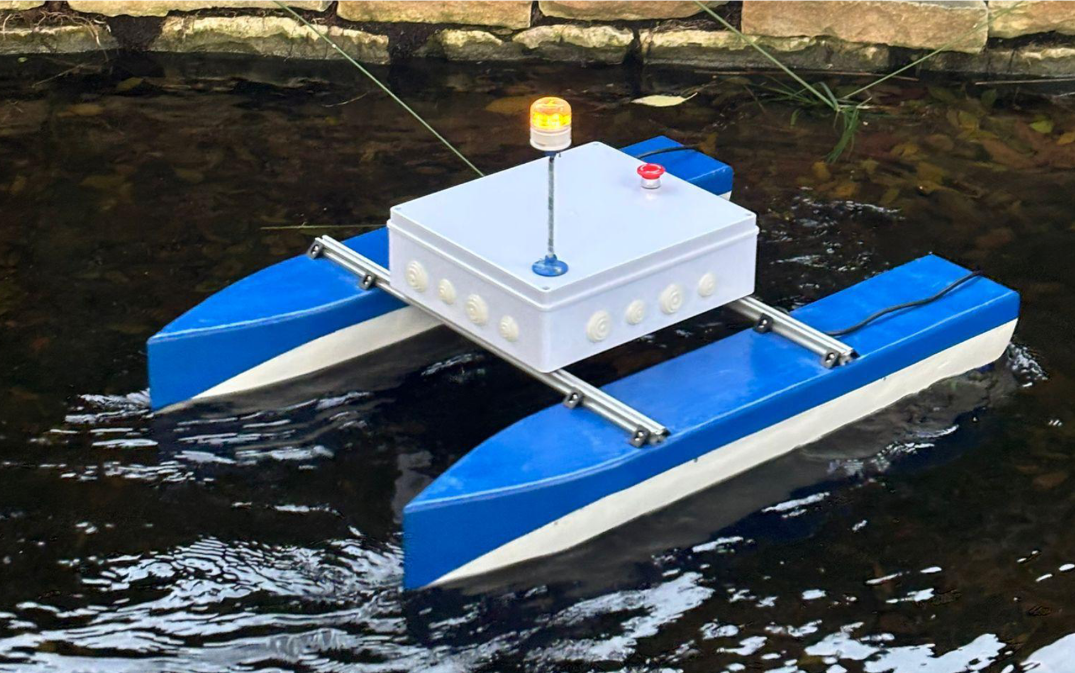
\includegraphics[width=0.5\linewidth]{figuras/usv-francisco.png}
    \caption[Estrutura do \gls{usv}]{Estrutura do \gls{usv} \cite{catamara-telecomandado}}
    \label{fig:usv-francisco}
\end{figure}

Para este processo foi utilizada uma impressora Ender 3 de primeira geração, modificada com a adição de um eixo vertical de 1,5 metros, de forma a possibilitar a produção de peças de maior dimensão. O material escolhido foi PLA, posteriormente reforçado com fibra de vidro, garantindo maior resistência mecânica e durabilidade em ambiente marítimo. 

No centro da estrutura foi instalada uma caixa estanque, destinada a albergar a eletrónica responsável pelo controlo do \gls{usv}, incluindo sensores, interfaces de comunicação e unidades de processamento. Esta caixa integra todos os elementos eletrónicos necessários ao funcionamento do sistema. 

A escolha da estrutura apresentada na Figura \ref{fig:usv-francisco} revela vantagens logísticas significativas. A Figura \ref{fig:pcb-esquematica-vs-real} compara o protótipo desenvolvido com o \gls{usv}-enautica1 da Sea2Future \cite{sea2future, sea2future2}, já ilustrado previamente na Figura \ref{fig:sea2future}.

\begin{figure}[H]
    \centering
    \begin{minipage}{0.39\linewidth}
        \centering
        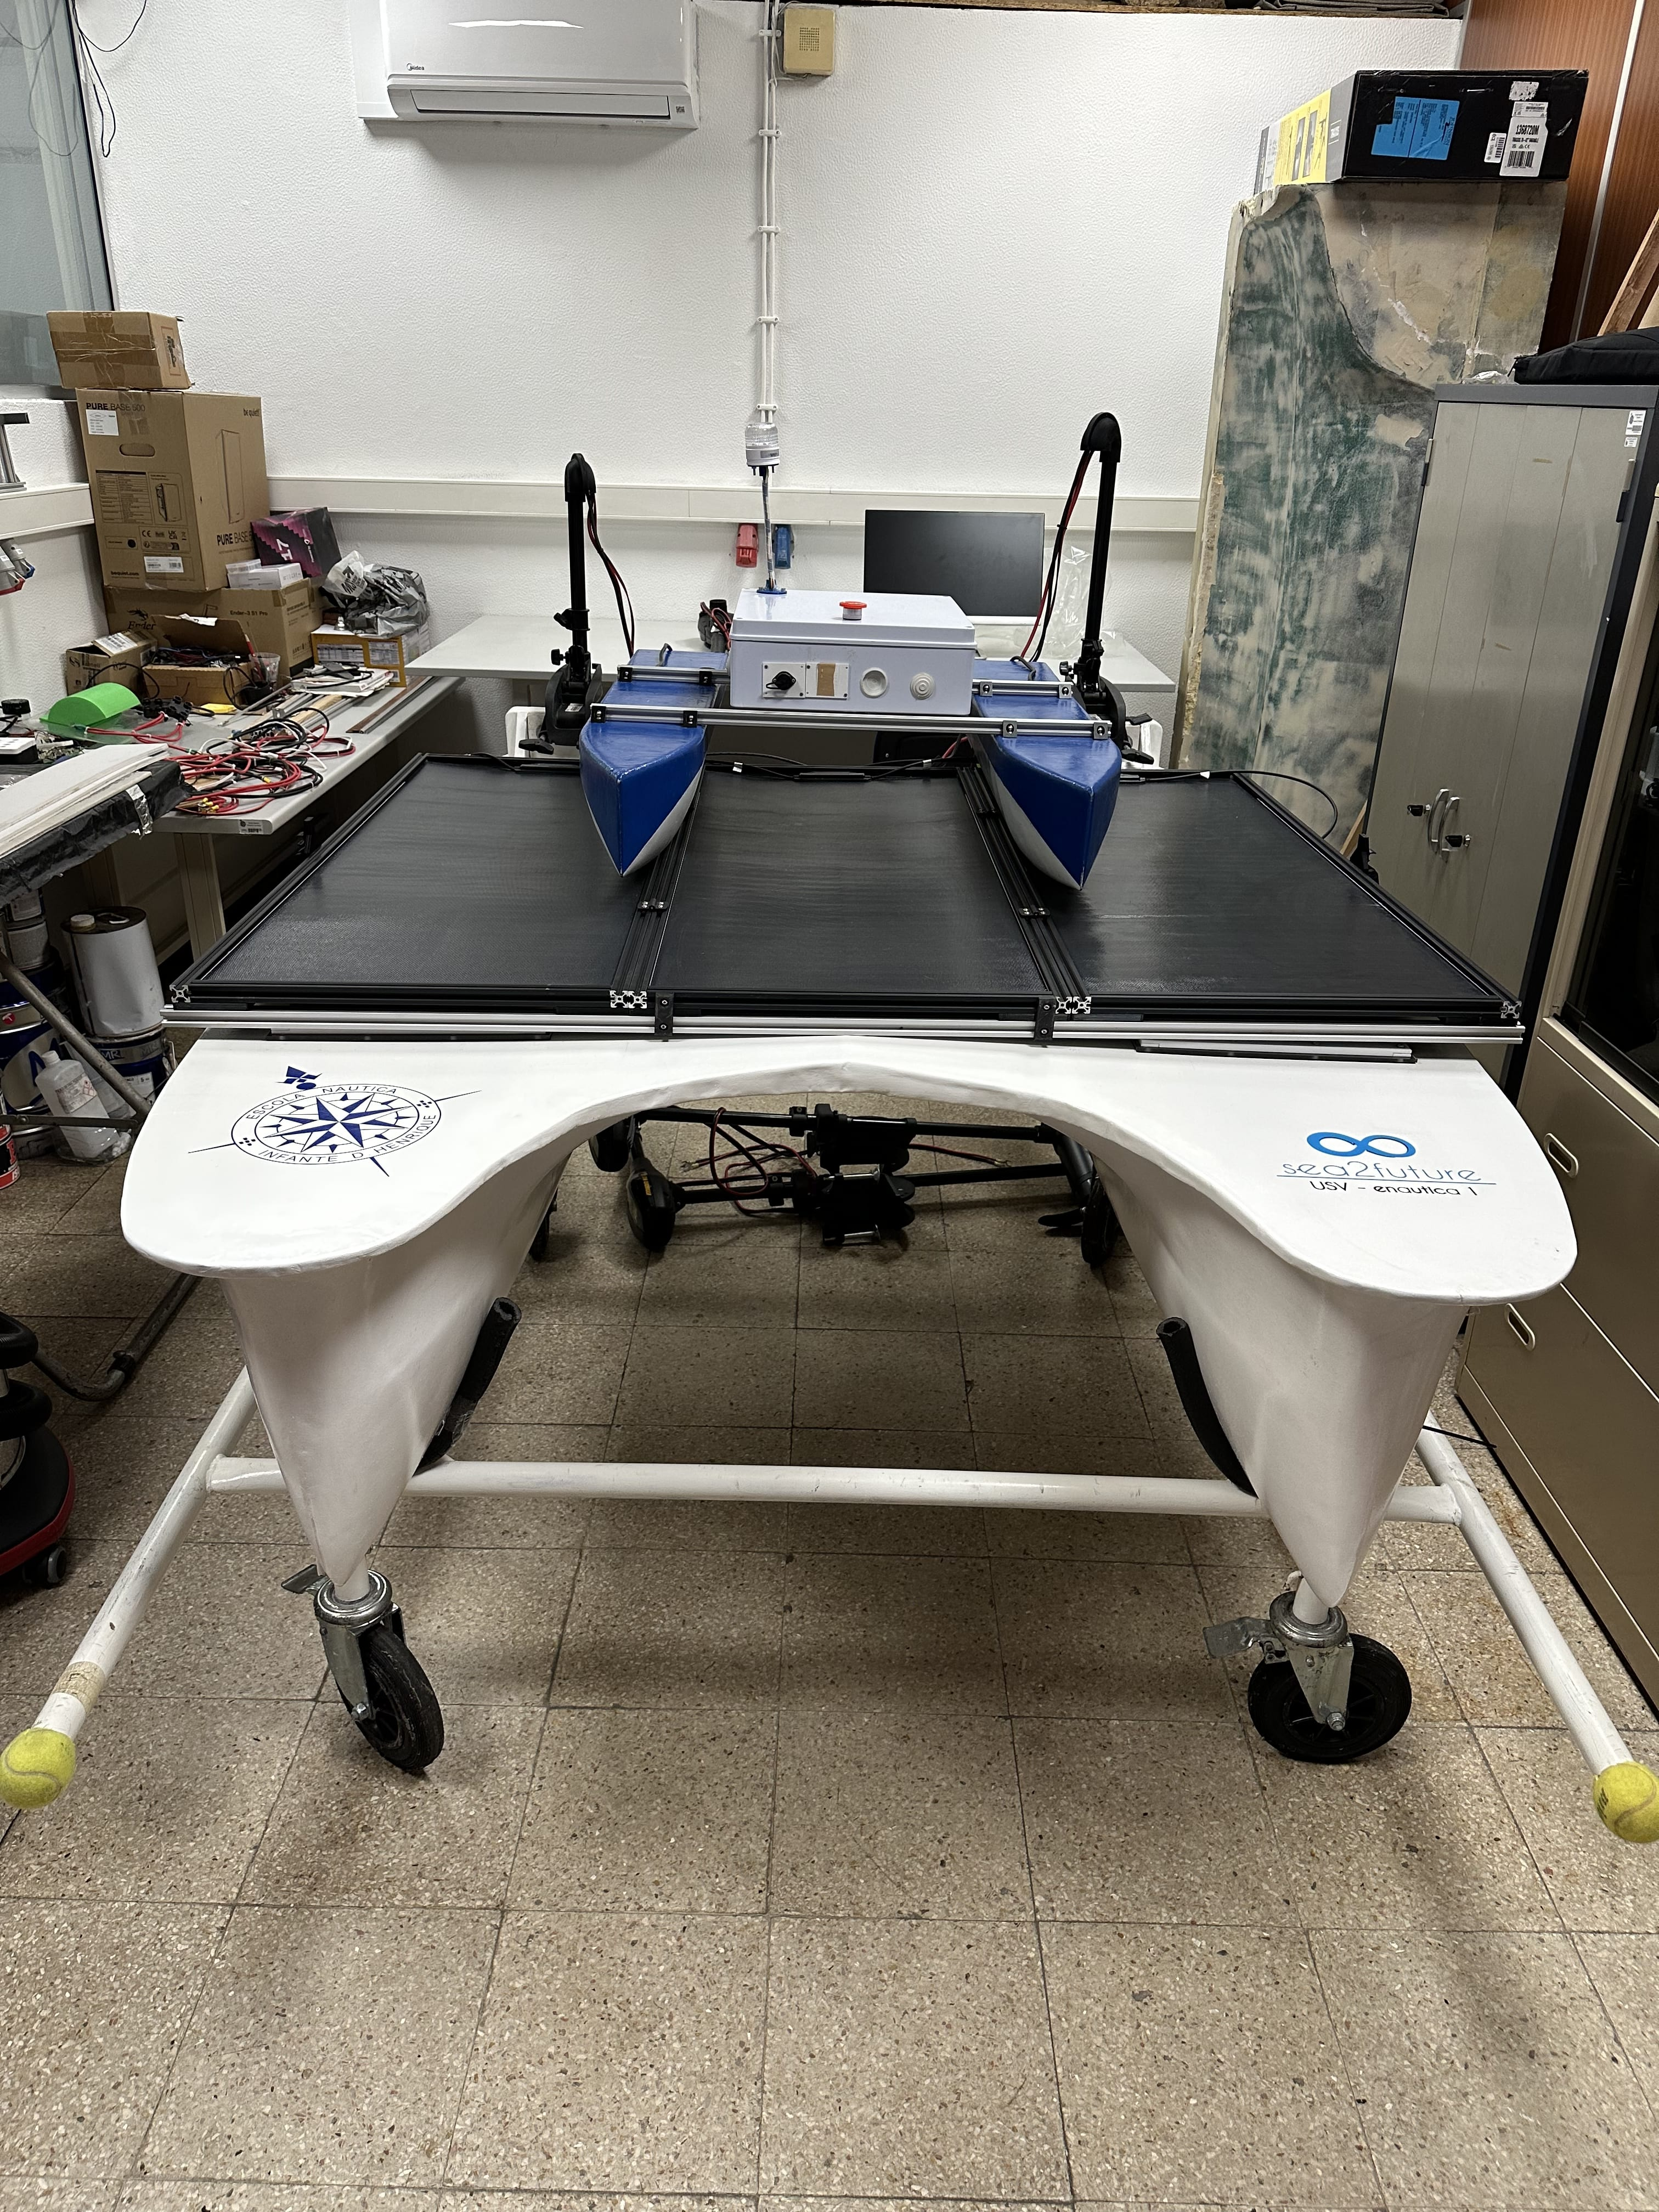
\includegraphics[height=6cm]{figuras/usv-1-2-1.jpg}
    \end{minipage}
    \hfill
    \begin{minipage}{0.59\linewidth}
        \centering
        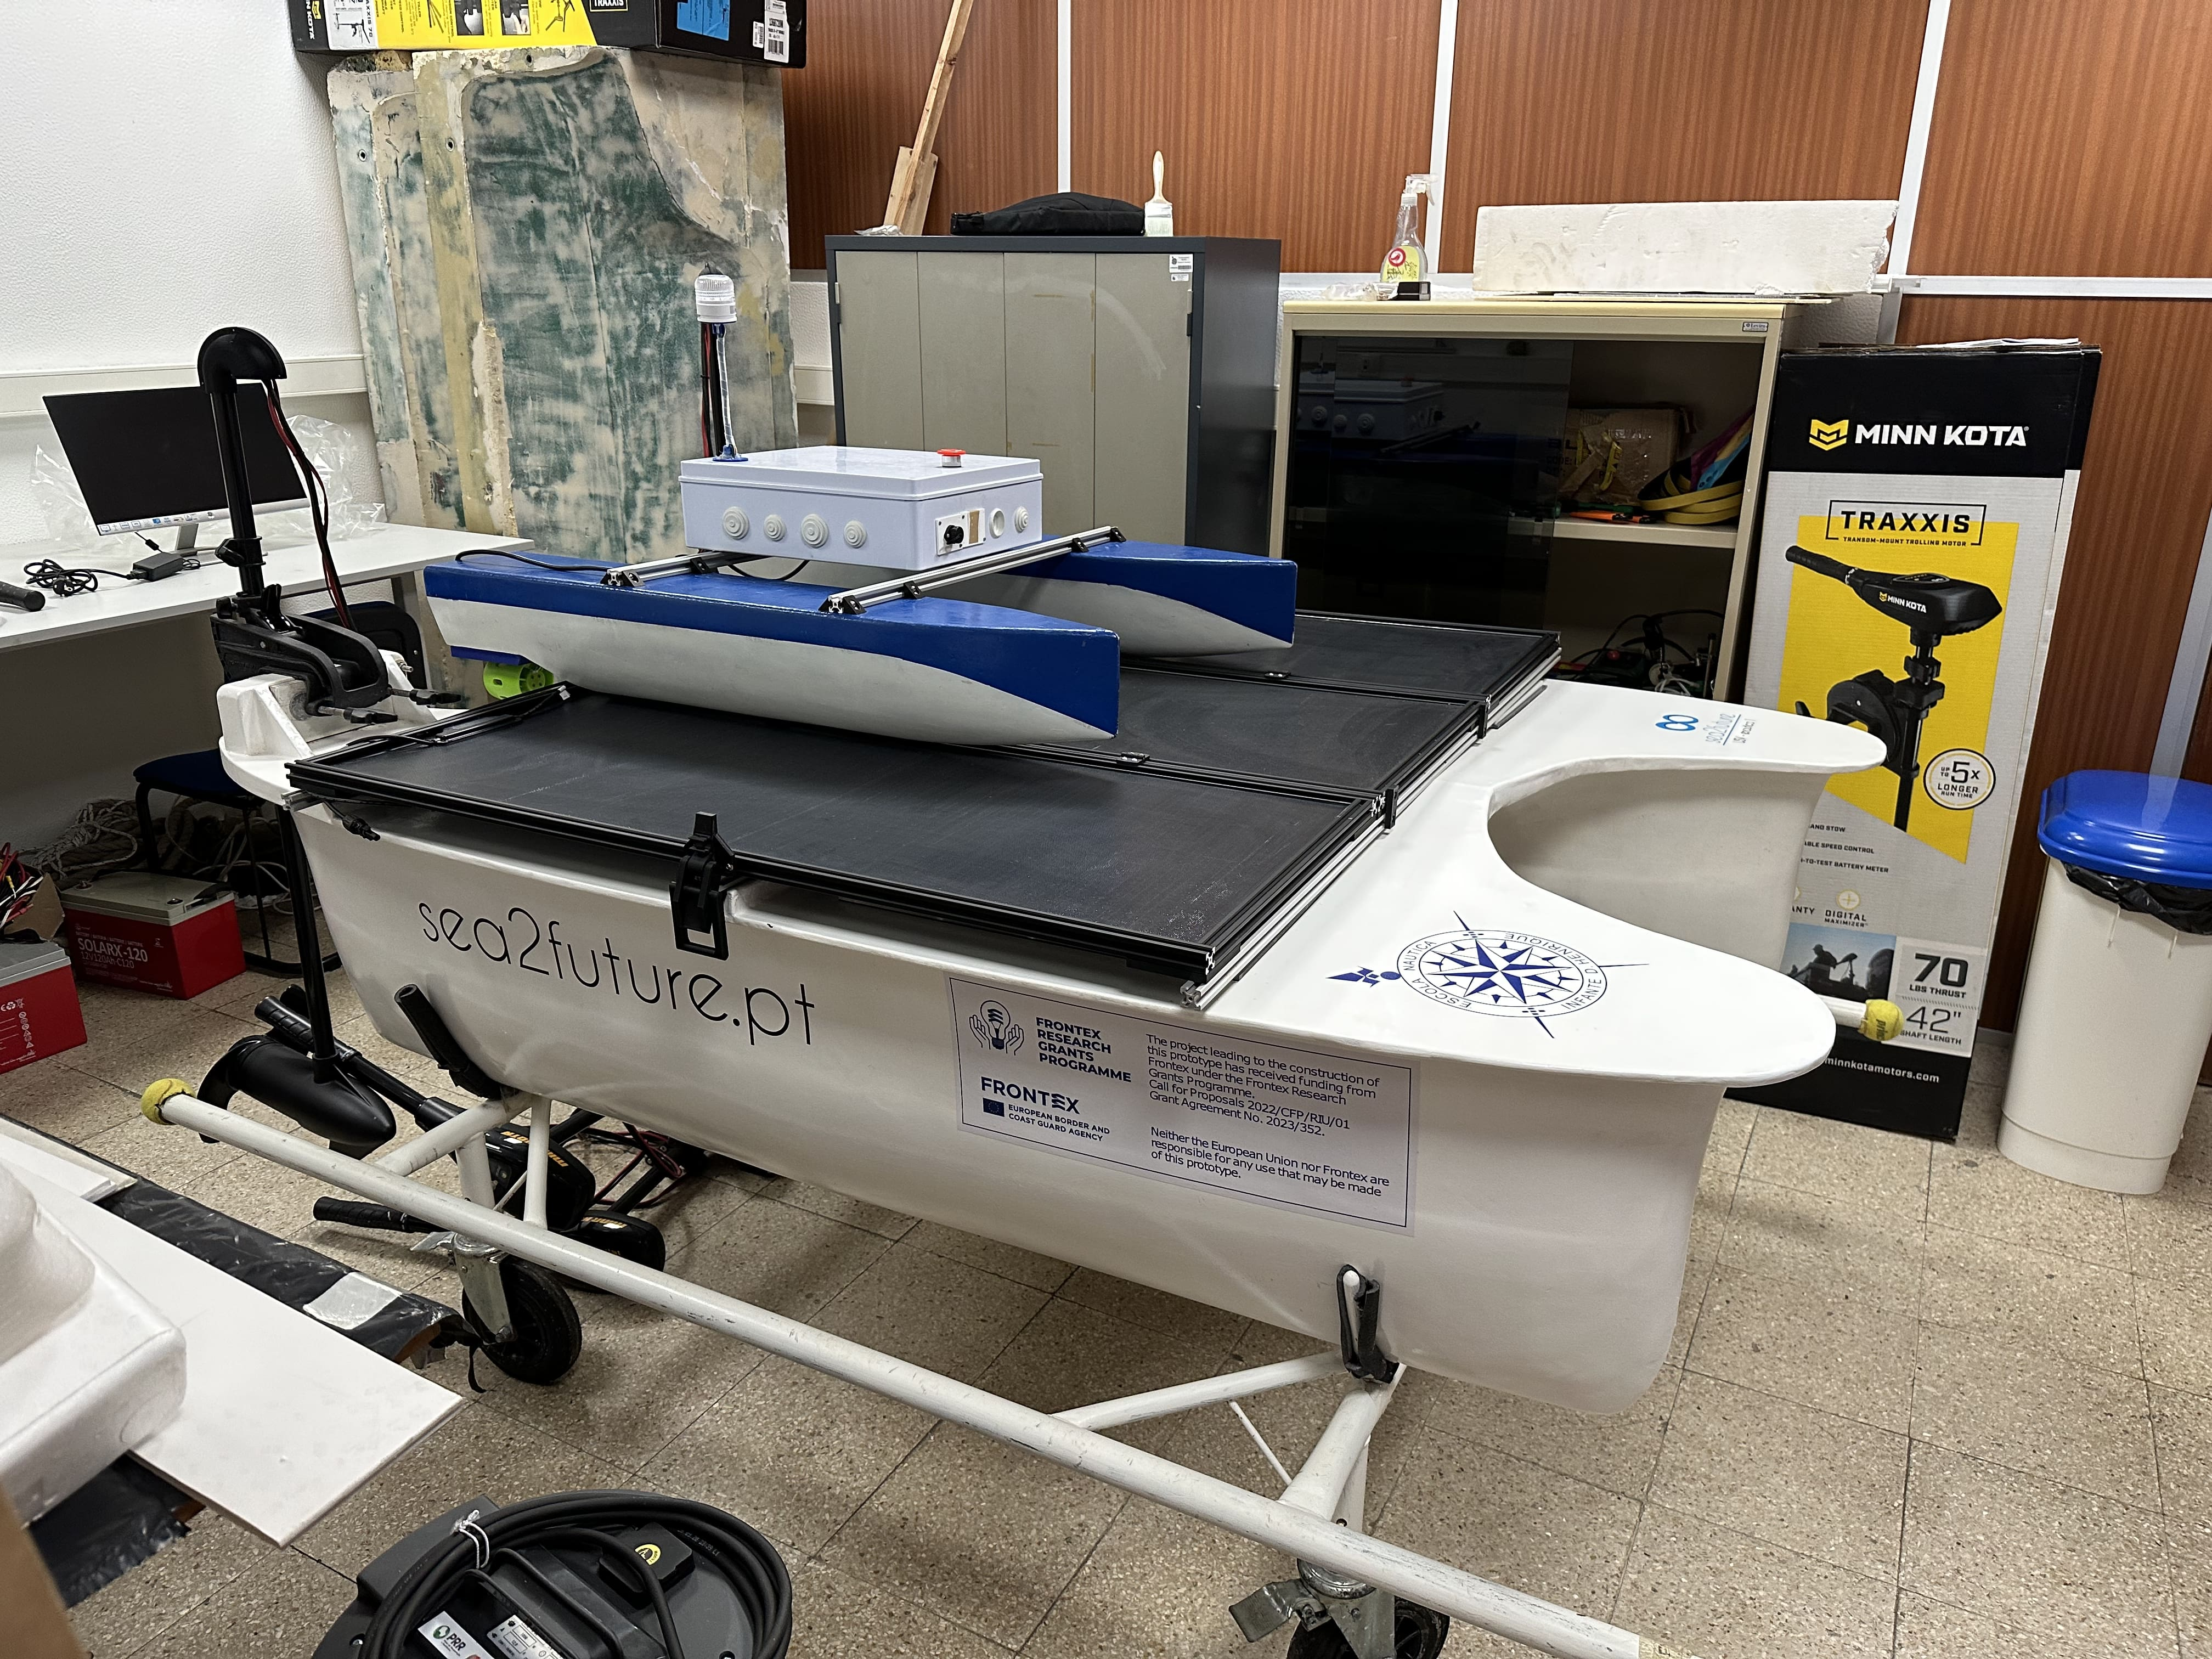
\includegraphics[height=6cm]{figuras/usv-1-2-2.jpg}
    \end{minipage}
    \caption{Comparação entre o \gls{usv}-enautica1 e o protótipo desenvolvido}
    \label{fig:pcb-esquematica-vs-real}
\end{figure}

O \gls{usv}-enautica1 apresenta dimensões e peso consideráveis, o que dificulta o seu transporte e limita a sua utilização em testes frequentes. Em contraste, a adoção de um catamarã mais pequeno e leve permite a realização de ensaios de navegação e validação de algoritmos de forma prática e acessível, assegurando maior portabilidade e facilidade de operação.  

É importante salientar que o \gls{usv}-enautica1 utiliza o mesmo tipo de controlo de motores \gls{pwm} integrados no protótipo desenvolvido neste \gls{tfm}, garantindo assim compatibilidade total com os procedimentos de controlo e validação aqui descritos. Esta correspondência tecnológica assegura que os resultados obtidos no protótipo são representativos e transferíveis para sistemas de maior escala desde que o controlo dos motores seja realizado de forma semelhante.

\section{Motores e Alimentação}
\label{sec:motor}

Tal como o robô didático descrito em \cite{didactic-robot-thesis}, o \gls{usv} desenvolvido neste trabalho recorre a motores para a sua propulsão. No entanto, em vez de motores \gls{dc} utilizados em protótipos educacionais, optou-se pela integração de propulsores subaquáticos de maior robustez, adequados ao ambiente de operação marítima. Estes propulsores, demonstrados na Figura \ref{fig:thrusters}, também conhecidos como \emph{thrusters}, são motores elétricos \emph{brushless} acoplados a hélices, cuja função é gerar empuxo ao movimentar o fluido envolvente (água), permitindo o deslocamento da embarcação.

\begin{figure}[H]
    \centering
    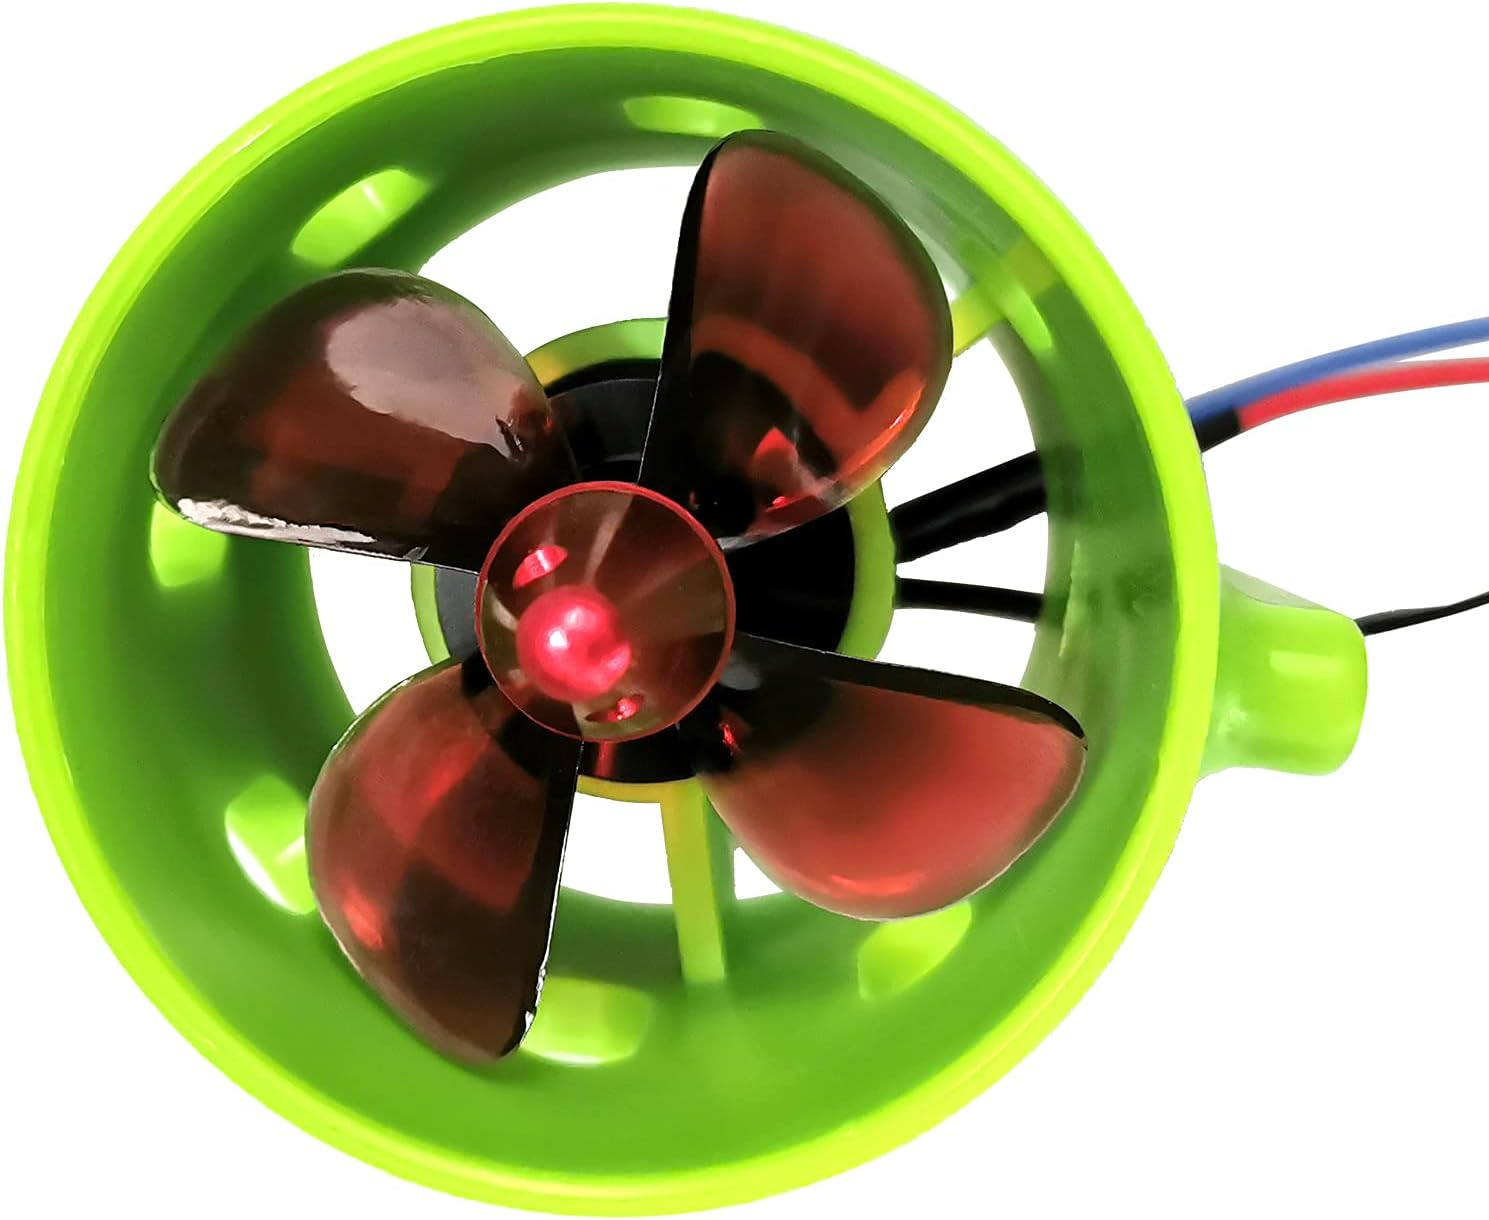
\includegraphics[width=0.33\linewidth]{figuras/thrusters.jpg}
    \caption{Propulsores \emph{brushless} utilizados no \gls{usv}}
    \label{fig:thrusters}
\end{figure}

% empuxo: força de propulsão gerada por um motor/hélice ao mover um fluido
Para este projeto foram selecionados os propulsores U01 \cite{apisqueen-underwater-thruster}, concebidos para aplicações em veículos de superfície e submersíveis de pequena escala. Estes motores operam numa faixa de tensão de 12 a 16 V, com uma potência nominal de 200 W, proporcionando até 2 kgf de empuxo em ambos os sentidos de rotação, uma vez que o seu controlador eletrónico (\gls{esc}) permite controlo bidirecional. Esta característica é essencial para o \gls{usv}, uma vez que garante a manobrabilidade necessária tanto para navegação em linha reta como para rotações em torno do próprio eixo permitindo mudar a direção da embarcação.

Em termos de integração elétrica, como ilustrado na Figura \ref{fig:bat-thruster}, cada motor é alimentado por uma bateria de 12 V de elevada capacidade, de forma a suportar a potência exigida e garantir autonomia de operação durante missões prolongadas. A escolha de propulsores \emph{brushless} deve-se a várias vantagens face aos motores \gls{dc} convencionais: maior eficiência energética, menor desgaste mecânico devido à ausência de escovas, capacidade de fornecer binário elevado a baixas rotações e maior fiabilidade em condições ambientais adversas, como a exposição contínua à água.

Adicionalmente, o sistema de controlo utiliza sinais de \gls{pwm} gerados pelo microcontrolador principal, que são interpretados pelo \gls{esc} de cada motor. Este mecanismo permite ajustar de forma contínua a velocidade e o sentido de rotação, possibilitando manobras precisas, tais como mudanças bruscas de direção ou movimentos de baixa velocidade em ambientes restritos.

A adoção de dois propulsores oferece um equilíbrio entre simplicidade e manobrabilidade, permitindo que o \gls{usv} execute translações e rotações sem necessidade de sistemas de direção adicionais. Contudo, a arquitetura do sistema foi concebida para ser escalável, suportando até quatro propulsores, caso seja necessário aumentar a estabilidade, a potência de propulsão ou a capacidade de operação em cenários marítimos mais exigentes.

\begin{figure}[H]
    \centering
    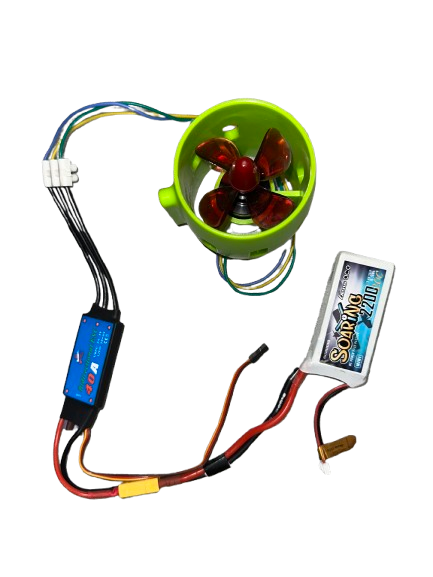
\includegraphics[width=0.5\linewidth, angle=-90]{figuras/IMG_4420-removebg-preview.png}
    \caption{Integração elétrica dos propulsores}
    \label{fig:bat-thruster}
\end{figure}

Para aplicações que exijam maior potência, podem ser utilizados motores mais robustos, como o Endura C2 \cite{datasheet-endura-c2} presentes no \gls{usv}-enautica1 da Sea2Future \cite{sea2future} \cite{sea2future2} e ilustrados tanto na Figura \ref{fig:sea2future} como na Figura \ref{fig:endura-c2}.

\begin{figure}[H]
    \centering
    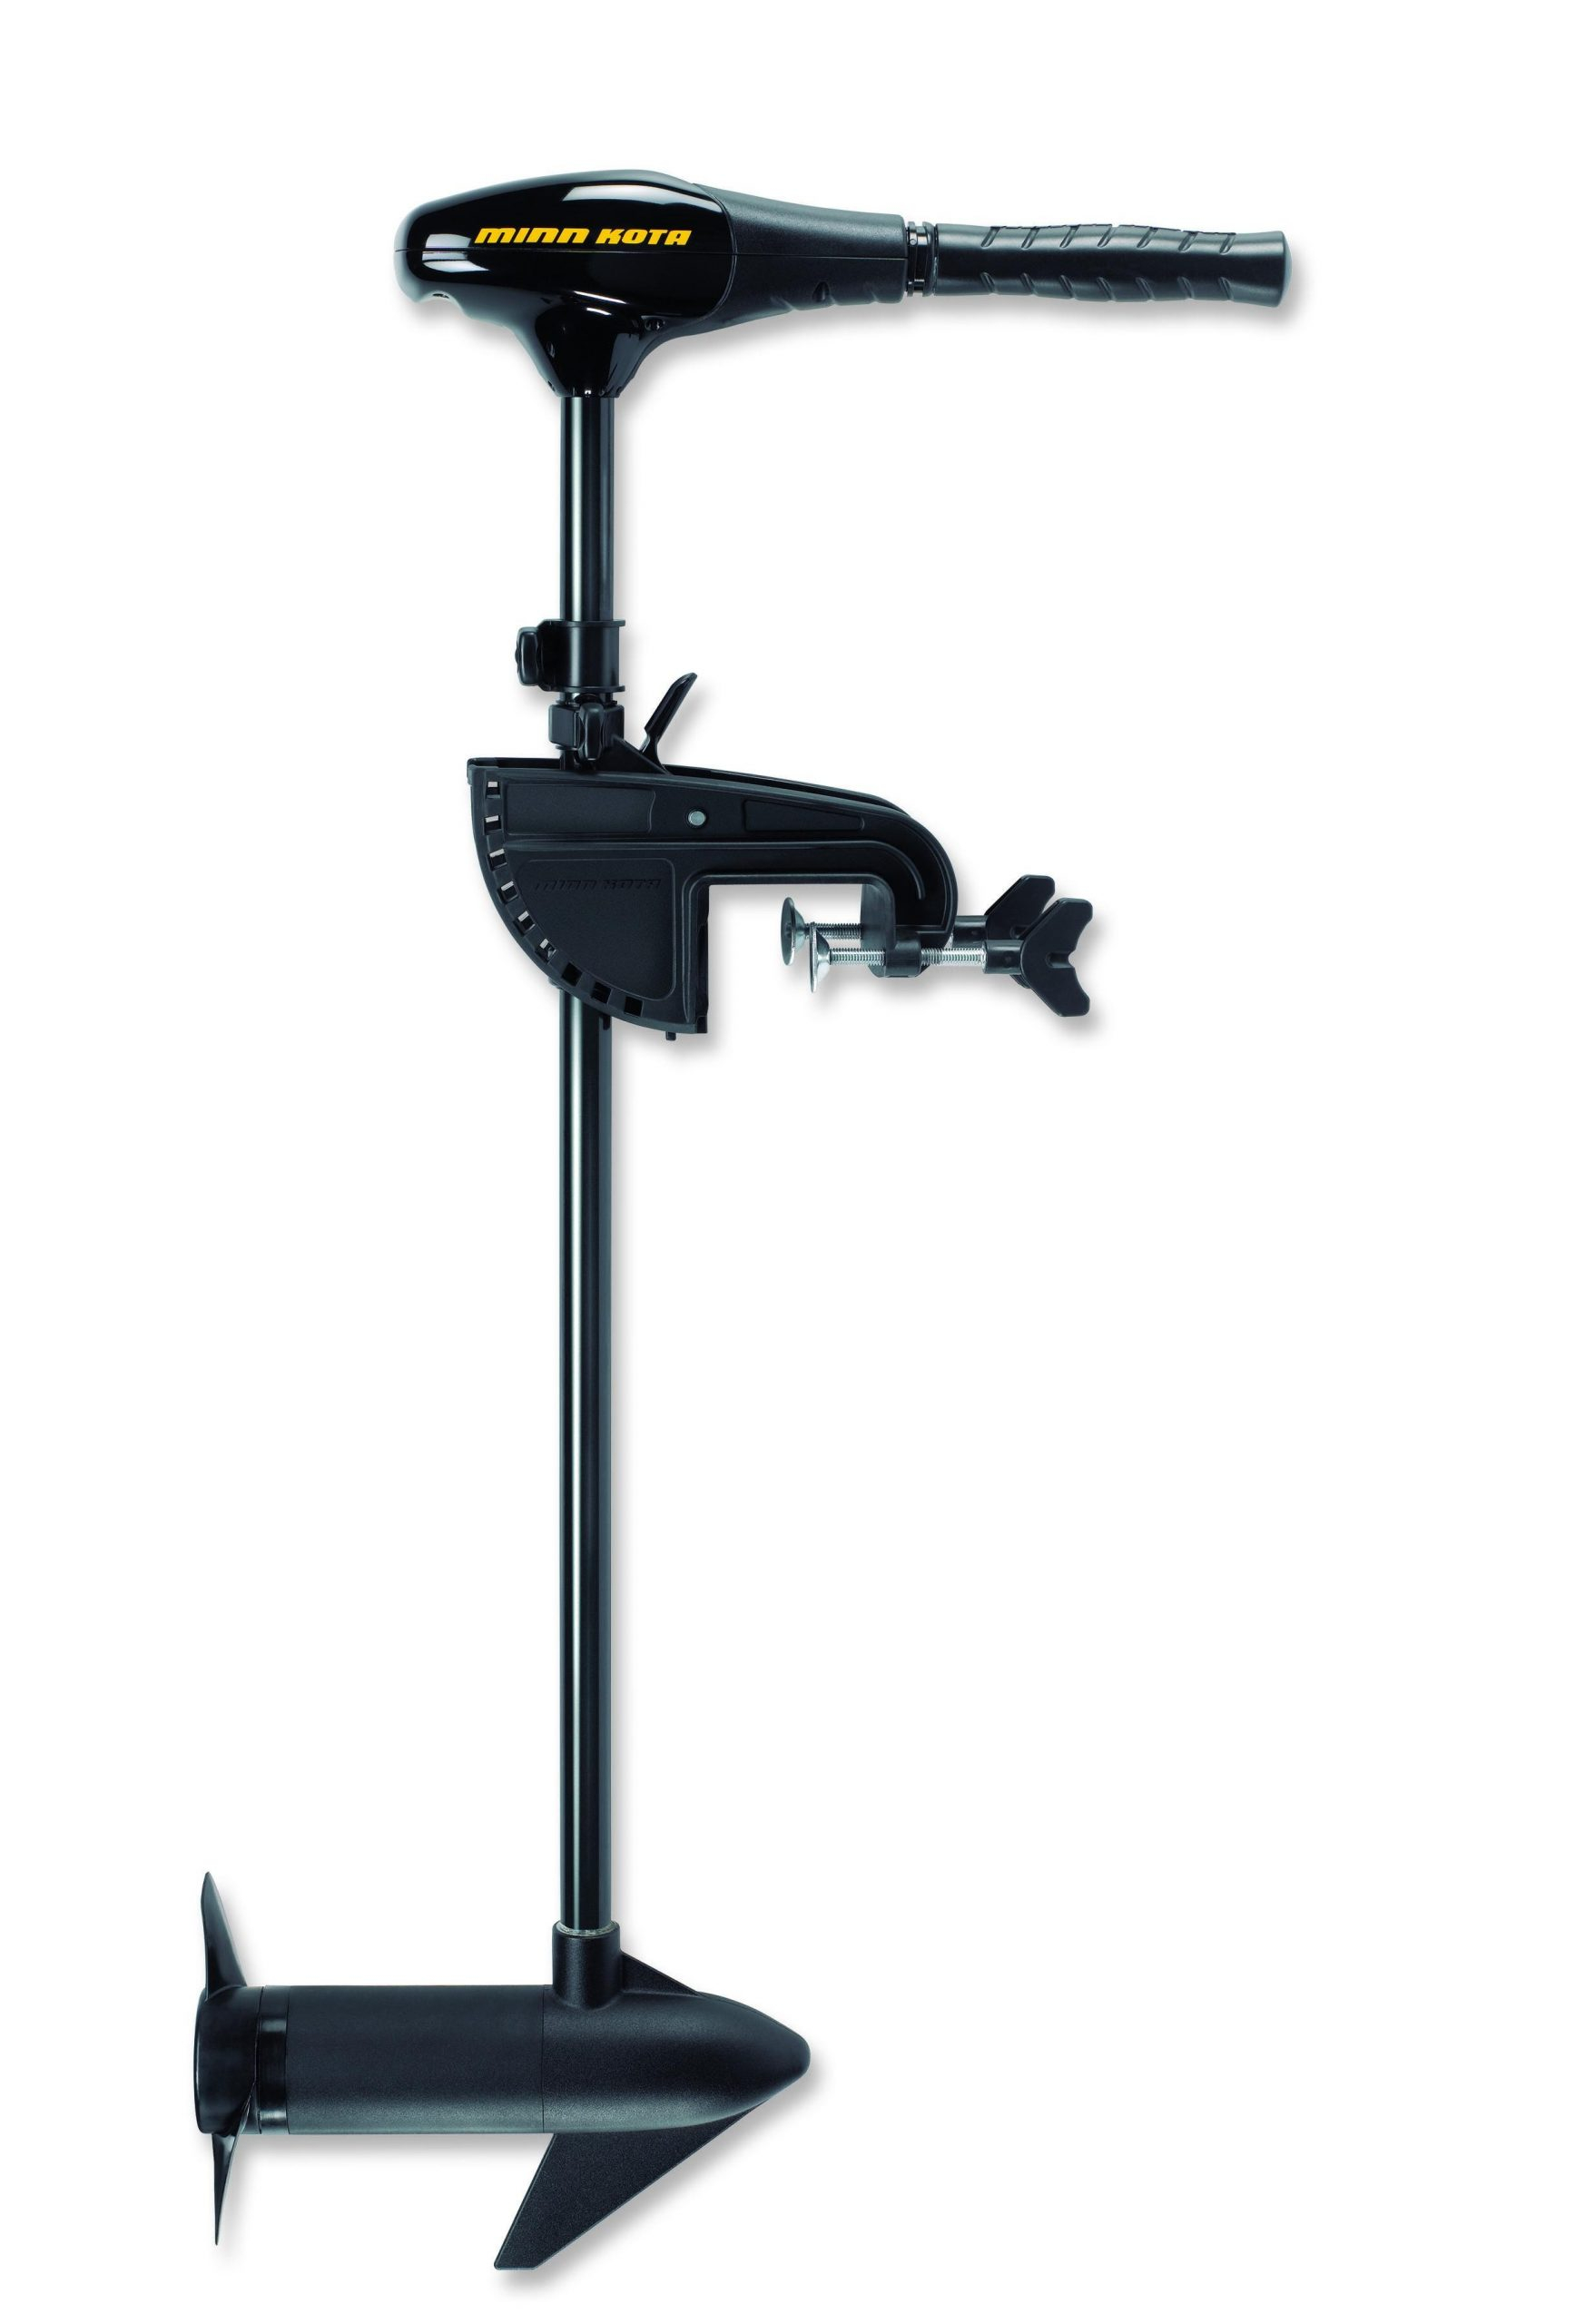
\includegraphics[width=0.33\linewidth]{figuras/endura-c2.jpg}
    \caption[Propulsores Endura C2]{Propulsores Endura C2 \cite{datasheet-endura-c2}}
    \label{fig:endura-c2}
\end{figure}

Os Endura C2 \cite{datasheet-endura-c2} requerem uma corrente de 30 A e, à semelhança dos propulsores utilizados neste \gls{tfm}, são alimentados por uma bateria externa de 12 V, garantindo a potência necessária para suportar missões mais exigentes em termos de velocidade e resistência.

\section{\acrfull{esc}}
\label{sec:esc}

O \acrfull{esc} é o componente responsável por controlar o funcionamento dos motores \emph{brushless} utilizados no \gls{usv}. Este dispositivo converte o sinal de comando proveniente do microcontrolador em impulsos elétricos adequados para alimentar as bobinas do motor, garantindo a regulação da sua velocidade e direção de rotação.

A Figura \ref{fig:pwm-sinal} apresenta a forma de onda do sinal de \gls{pwm} aplicado ao \gls{esc} para controlar os \emph{thursters}.implementação. A Figura 4.3 apresenta a forma de onda do sinal de \gls{pwm} descrito.

O princípio de funcionamento baseia-se na utilização de sinais de \gls{pwm} enviados pelo microcontrolador. Estes sinais consistem em pulsos periódicos cuja largura (duração em microssegundos) determina a resposta do motor \cite{didactic-robot-thesis}. Tipicamente, um sinal com largura de $1000\,\mu s$ (linha azul da Figura \ref{fig:pwm-sinal}) corresponde à velocidade mínima no sentido inverso, $1500\,\mu s$ (linha laranja da Figura \ref{fig:pwm-sinal}) corresponde ao ponto neutro, no qual o motor permanece parado, e $2000\,\mu s$ (linha verde da Figura \ref{fig:pwm-sinal}) corresponde à velocidade máxima no sentido direto. A partir deste ponto central, a largura do pulso varia de forma simétrica: valores inferiores a $1500\,\mu s$ comandam rotações no sentido inverso com velocidade crescente à medida que a largura do pulso diminui, enquanto valores superiores a $1500\,\mu s$ comandam rotações no sentido direto com velocidade crescente à medida que a largura do pulso aumenta. A frequência habitual do sinal é de $50\,Hz$, o que significa que cada período tem $20000\,\mu s$. Este padrão segue a mesma lógica dos sinais de controlo usados em servomotores, o que facilita a sua implementação e utilização de controladores \emph{standard} de radio controle utilizado em modelismo. 

\begin{figure}[H]
    \centering
    % Substituir pelo diagrama do sinal PWM (1000 \(\mu s\), 1500 \(\mu s\), 2000 \(\mu s\))
    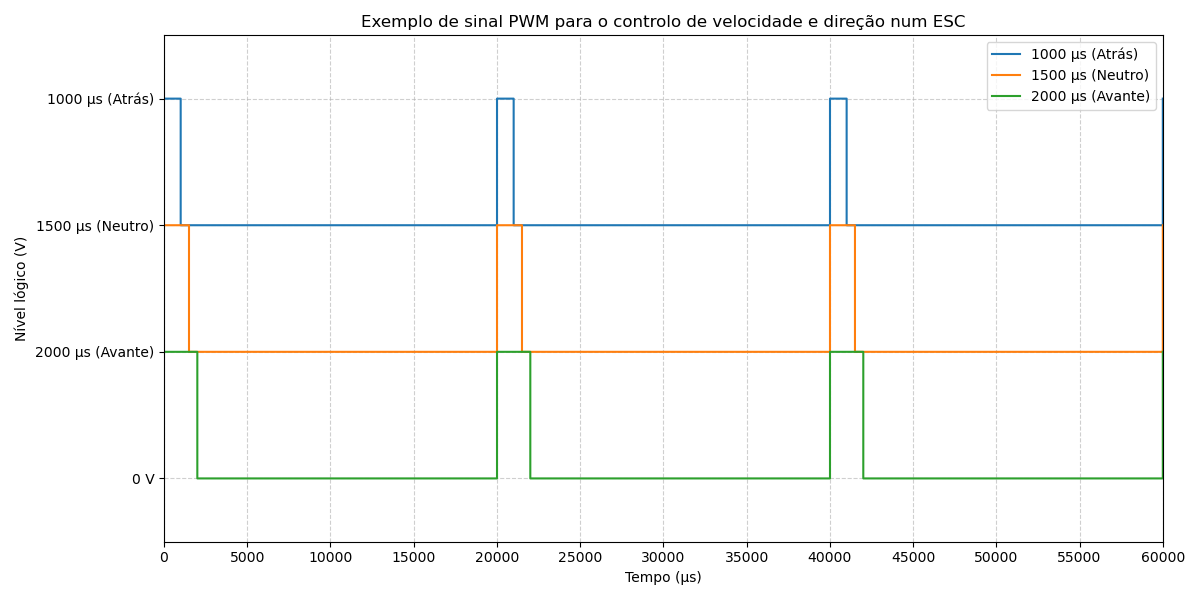
\includegraphics[width=1\linewidth]{figuras/pwm_us.png}
    \caption{Exemplo de sinal \gls{pwm} para o controlo de velocidade e direção num \gls{esc}}
    \label{fig:pwm-sinal}
\end{figure}

Antes de os motores poderem ser utilizados, o \gls{esc} necessita de ser armado, este processo consiste na aplicação de uma sequência de sinais de inicialização que confirmam a ligação entre o controlador e o motor, garantindo que este não entra em funcionamento acidentalmente. No caso em estudo, este procedimento envolve enviar inicialmente um sinal de largura mínima (por exemplo, $1000\,\mu s$) durante 2 segundos, seguido da transição para a largura correspondente ao ponto neutro ($1500\,\mu s$). Apenas após esta sequência o \gls{esc} considera o sistema pronto a operar, emitindo normalmente sinais sonoros característicos que confirmam o estado de prontidão.

O controlo bidirecional da rotação é assegurado pelo próprio \gls{esc}, que interpreta os sinais de \gls{pwm} acima e abaixo do ponto neutro. Assim:

\begin{itemize}
    \item Pulsos inferiores a $1500\,\mu s$ comandam a rotação no sentido inverso (atrás);
    \item Pulsos superiores a $1500\,\mu s$ comandam a rotação no sentido direto (frente).
\end{itemize}

Este mecanismo elimina a necessidade de sistemas mecânicos de inversão de polaridade, uma vez que o \gls{esc} efetua digitalmente a comutação das fases do motor \emph{brushless}. A grande vantagem desta abordagem é a elevada precisão no controlo da velocidade, associada a uma resposta rápida e eficiente, fatores críticos para a manobrabilidade do \gls{usv} em cenários marítimos complexos.

Em síntese, o \gls{esc} desempenha um papel central no sistema de propulsão: traduz os comandos enviados pelo microcontrolador em potência controlada para os motores, garante a segurança durante a inicialização através do processo de armamento, e possibilita a rotação bidirecional através da modulação do sinal \gls{pwm}.

\section{Sensores} 
\label{sec:sensores}

A operação autónoma de um \gls{usv} depende fortemente da disponibilidade de sensores capazes de fornecer medições fiáveis sobre a sua posição, movimento e orientação. Estes dados constituem a base para o controlo de navegação, permitindo não apenas o seguimento rigoroso de rotas previamente definidas, mas também a correção dinâmica de desvios causados por correntes, ondas ou vento.  

No protótipo desenvolvido, a arquitetura de sensorização foi concebida de forma modular, possibilitando a integração e substituição de sensores de maneira independente, sem comprometer a funcionalidade global. Esta abordagem garante escalabilidade e flexibilidade, permitindo adaptar o sistema a diferentes cenários operacionais ou evoluir para missões com requisitos mais complexos.  

Entre os sensores integrados, destacam-se dois elementos centrais. O primeiro é o \acrfull{imu}, responsável por medir aceleração, velocidade angular e intensidade do campo magnético, permitindo calcular com elevada precisão a orientação do veículo nos três eixos principais (\emph{yaw}, \emph{pitch} e \emph{roll}). O segundo é o recetor \acrfull{gps}, que fornece a posição geográfica absoluta em coordenadas de latitude e longitude, constituindo a referência essencial para a definição e seguimento de \emph{waypoints}.  

O uso combinado destes dois sensores permite mitigar as limitações individuais de cada um: enquanto o \gls{imu} fornece dados de orientação com elevada taxa de atualização, mas sofre de erro acumulado, o \gls{gps} disponibiliza medições absolutas de posição, embora com menor frequência e suscetíveis a erros momentâneos. Assim, a fusão de dados provenientes de ambos os sensores garante maior precisão, robustez e fiabilidade na estimativa da trajetória do \gls{usv}.  

As subseções seguintes apresentam em detalhe a integração do \acrfull{imu} (Subsecção \ref{subsec:imu}) e do recetor \acrfull{gps} (Subsecção \ref{subsec:gps}), descrevendo os princípios de funcionamento, a configuração adotada e o contributo de cada sensor para a arquitetura global de navegação.


\subsection{\acrfull{imu}} \label{subsec:imu}

O \gls{imu} é um dispositivo fundamental para medir a orientação e o movimento do \gls{usv}. Este sensor combina três subsistemas principais: acelerómetros, giroscópios e magnetómetros, que medem, respetivamente, a aceleração linear, a velocidade angular e a intensidade do campo magnético terrestre. A partir destes dados é possível calcular os ângulos de guinada (\emph{yaw}), arfagem (\emph{pitch}) e rotação (\emph{roll}), que descrevem a orientação tridimensional da embarcação, como ilustrado na Figura~\ref{fig:pitch-roll-yaw}.

\begin{figure}[H]
    \centering
    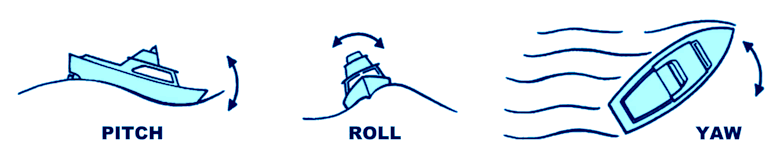
\includegraphics[height=0.2\linewidth]{figuras/Pitch-Roll-Yaw.png}
    \caption[Representação do \emph{yaw}, \emph{pitch} e \emph{roll} numa embarcação]{Representação do \emph{yaw}, \emph{pitch} e \emph{roll} numa embarcação \cite{imagem-yaw-pitch-roll}}
    \label{fig:pitch-roll-yaw}
\end{figure}

O ângulo de \emph{yaw} representa a rotação em torno do eixo vertical, sendo responsável pela direção do movimento da embarcação. O \emph{pitch} indica a inclinação para a frente e para trás, refletindo a estabilidade longitudinal face às ondas. Por sua vez, o \emph{roll} mede a inclinação lateral, relacionada com a estabilidade transversal do \gls{usv}.

No âmbito deste projeto foram avaliadas duas opções de sensores \gls{imu}: o MPU6050 e o MPU9250. O MPU6050 fornece medições em seis eixos (aceleração e velocidade angular), enquanto o MPU9250 adiciona um magnetómetro, totalizando nove graus de liberdade. Este último permite medições absolutas de orientação, compensando o erro acumulado do giroscópio, e foi por isso selecionado para o sistema.

A partir dos dados fornecidos por este sensor é possível calcular numericamente os ângulos de orientação do \gls{usv}. As equações seguintes descrevem o processo de cálculo de \emph{yaw}, \emph{pitch} e \emph{roll}, com explicação detalhada dos parâmetros envolvidos.

\subsubsection{\emph{Yaw} (\(\Psi\))}

O ângulo de guinada (\emph{yaw}, \(\Psi\)) indica a orientação horizontal da embarcação em relação ao norte magnético (Figura~\ref{fig:yaw}). É calculado a partir das medições do magnetómetro corrigidas pela inclinação do sensor, determinada pelos ângulos de \emph{pitch} (\(\Theta\)) e \emph{roll} (\(\Phi\)).

\begin{figure}[H]
    \centering
    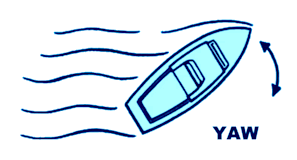
\includegraphics[height=0.2\linewidth]{figuras/Yaw.png}
    \caption[Representação do \emph{yaw} numa embarcação]{Representação do \emph{yaw} numa embarcação (Adaptada de \cite{imagem-yaw-pitch-roll})}
    \label{fig:yaw}
\end{figure}

O primeiro passo consiste em compensar a inclinação do sensor nos eixos \(x\) e \(z\), conforme a Equação~\ref{eq:mx_prime}:

\begin{equation}
    m_x' = m_x \cos(\Theta) + m_z \sin(\Theta)
    \label{eq:mx_prime}
\end{equation}

onde \(m_x\) e \(m_z\) são as componentes do campo magnético medidas pelo magnetómetro nos respetivos eixos, e \(\Theta\) representa o ângulo de \emph{pitch}.  

De seguida, calcula-se o valor corrigido de \(m_y'\), conforme a Equação~\ref{eq:my_prime}:

\begin{equation}
    m_y' = m_x \sin(\Phi) \sin(\Theta) + m_y \cos(\Phi) - m_z \sin(\Phi) \cos(\Theta)
    \label{eq:my_prime}
\end{equation}

em que \(m_y\) é a componente do campo magnético no eixo \(y\), e \(\Phi\) corresponde ao ângulo de \emph{roll}.  

Com as componentes corrigidas \(m_x'\) e \(m_y'\), o ângulo de \emph{yaw} é obtido através da função trigonométrica \(\arctan2\), conforme a Equação~\ref{eq:yaw}:

\begin{equation}
    \Psi = \arctan2(-m_y', m_x')
    \label{eq:yaw}
\end{equation}

Esta função assegura que o resultado é atribuído ao quadrante correto, produzindo um ângulo contínuo entre \(-180^\circ\) e \(180^\circ\).

\subsubsection{\emph{Pitch} (\(\Theta\))}

O ângulo de arfagem (\emph{pitch}, \(\Theta\)) mede a inclinação do \gls{usv} no eixo longitudinal, como mostrado na Figura~\ref{fig:pitch}. É obtido diretamente a partir das leituras do acelerómetro, considerando as acelerações lineares \(a_x\), \(a_y\) e \(a_z\) nos três eixos principais.

\begin{figure}[H]
    \centering
    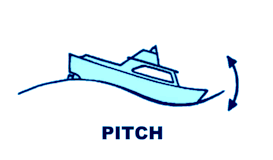
\includegraphics[height=0.2\linewidth]{figuras/Pitch.png}
    \caption[Representação do \emph{pitch} numa embarcação]{Representação do \emph{pitch} numa embarcação (Adaptada de \cite{imagem-yaw-pitch-roll})}
    \label{fig:pitch}
\end{figure}

O cálculo é dado pela Equação~\ref{eq:pitch}:

\begin{equation}
    \Theta = \arcsin{\left(\frac{-a_x}{\sqrt{a_x^2 + a_y^2 + a_z^2}}\right)}
    \label{eq:pitch}
\end{equation}

Nesta expressão, \(a_x\), \(a_y\) e \(a_z\) correspondem às componentes da aceleração linear medidas pelo acelerómetro. A normalização pelo termo \(\sqrt{a_x^2 + a_y^2 + a_z^2}\) assegura que o cálculo é independente da intensidade total da aceleração, considerando apenas a direção relativa da gravidade.

\subsubsection{\emph{Roll} (\(\Phi\))}

O ângulo de rotação (\emph{roll}, \(\Phi\)) representa a inclinação lateral da embarcação em torno do eixo longitudinal, sendo crítico para avaliar a estabilidade transversal (Figura~\ref{fig:roll}).

\begin{figure}[H]
    \centering
    
\includegraphics[height=0.2\linewidth]{figuras/Roll.png}
    \caption[Representação do \emph{roll} numa embarcação]{Representação do \emph{roll} numa embarcação (Adaptada de \cite{imagem-yaw-pitch-roll})}
    \label{fig:roll}
\end{figure}

Este ângulo é determinado pela Equação~\ref{eq:roll}:

\begin{equation}
    \Phi = \arctan2(a_y, a_z)
    \label{eq:roll}
\end{equation}

onde \(a_y\) e \(a_z\) são as acelerações medidas nos eixos transversal e vertical, respetivamente. A função \(\arctan2\) é utilizada para garantir que o ângulo resultante é atribuído ao quadrante correto, permitindo distinguir entre inclinações à esquerda e à direita.  

Em conjunto, as Equações~\ref{eq:mx_prime} a~\ref{eq:roll} permitem calcular de forma precisa a orientação instantânea do \gls{usv}, integrando as leituras do magnetómetro e do acelerómetro para compensar erros e variações dinâmicas durante a navegação.

\subsection{\acrfull{gps}}
\label{subsec:gps}

O \gls{gps} é uma tecnologia amplamente utilizada para a determinação da posição geográfica de objetos ou indivíduos em qualquer ponto do globo. Este sistema, desenvolvido inicialmente pelo Departamento de Defesa dos Estados Unidos, é constituído por uma constelação de satélites que transmitem sinais de rádio para dispositivos recetores na Terra. Estes sinais são processados para calcular coordenadas geográficas com elevada precisão, fornecendo informações cruciais em aplicações de navegação, monitorização e controlo de sistemas móveis, como veículos autónomos.

O funcionamento do \gls{gps} baseia-se no princípio da triangulação, tal como se pode observar na Figura \ref{fig:triangulacao}), onde pelo menos quatro satélites são necessários para determinar com precisão a posição de um recetor no espaço tridimensional (latitude, longitude e altitude). Cada satélite transmite sinais codificados contendo informações sobre a sua posição e o tempo exato em que o sinal foi enviado. O recetor \gls{gps} calcula o tempo que o sinal levou a chegar a partir de múltiplos satélites, determinando assim a distância de cada um. Com base nestes dados, a posição do recetor é triangulada. 

No caso do \gls{usv}, apenas são necessários três satélites, pois não é necessário determinar a altitude. Como o \gls{usv} opera na superfície da água, a sua posição é restrita a um plano bidimensional, considerando apenas latitude e longitude. Desta forma, a triangulação pode ser realizada com precisão utilizando apenas três satélites, simplificando o cálculo em relação a sistemas que requerem coordenadas tridimensionais.

\begin{figure}[H]
    \centering
    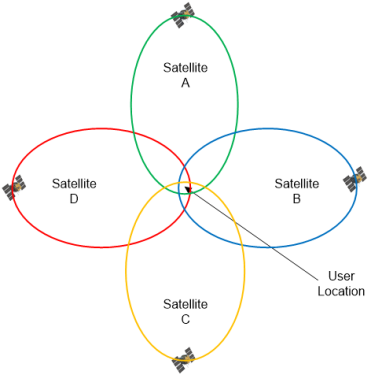
\includegraphics[width=0.33\linewidth]{figuras/lowdop.png}
    \caption[Triangulação do sinal \gls{gps}]{Triangulação do sinal \gls{gps} \cite{help-gps}}
    \label{fig:triangulacao}
\end{figure}

O sistema \gls{gps} depende de relógios atómicos precisos instalados nos satélites para garantir a sincronização temporal. Além disso, algoritmos avançados compensam erros causados por fatores como a atmosfera terrestre e o desvio orbital dos satélites.

Entre as principais vantagens do \gls{gps}, destacam-se a sua elevada precisão, que em condições ideais permite obter localizações com margens de erro de poucos metros, e a cobertura global, que garante funcionalidade em qualquer lugar do mundo, independentemente de fronteiras geográficas. Adicionalmente, o recetor \gls{gps} opera de forma passiva, recebendo sinais sem necessidade de os transmitir, o que contribui para a eficiência energética. A sua facilidade de integração em sistemas autónomos, como os \gls{usv} descritos neste \gls{tfm}, é também uma característica relevante.

Por outro lado, o \gls{gps} apresenta algumas limitações, como a dependência de visibilidade direta com os satélites, sendo o sinal frequentemente bloqueado por obstáculos como edifícios, montanhas, vegetação ou nuvêns densas. As condições atmosféricas, incluindo tempestades solares e interferências atmosféricas, podem comprometer a precisão do sistema. Além disso, o consumo energético do recetor, embora moderado, pode ser um desafio em dispositivos com baterias de capacidade limitada. Por fim, o \gls{gps} é vulnerável a interferências e bloqueios intencionais (\emph{jamming}), o que reduz a sua fiabilidade em situações críticas.

Apesar da possibilidade de utilizar apenas um \gls{imu} para estimar a posição e orientação do \gls{usv}, esta abordagem revela-se insuficiente em aplicações que exigem elevada precisão em trajetos extensos. O \gls{imu} utiliza sensores como acelerómetros e giroscópios para calcular deslocações relativas, mas está sujeito a deriva acumulada ao longo do tempo devido a erros nos sensores e no processamento de dados. A combinação com um \gls{gps} é, portanto, fundamental, uma vez que este fornece medições absolutas que corrigem a deriva inerente ao \gls{imu}, assegurando uma navegação fiável e precisa.  

Importa salientar que recetores \gls{gps} são tipicamente configurados e utilizados através de portas série (\gls{uart}), o que representa um desafio quando se pretende integrar múltiplos módulos num sistema que privilegia a comunicação via \gls{i2c}. No contexto deste \gls{tfm}, foi definido como requisito que todos os módulos comunicassem preferencialmente através do barramento \gls{i2c}, de modo a simplificar a arquitetura e reduzir o número de interfaces independentes no microcontrolador. Para alcançar este objetivo, foi integrado um conversor \gls{i2c}-\gls{uart} (SC16IS750), que atua como uma ponte entre os dois protocolos. Esta solução permitiu expandir o número de interfaces série disponíveis sem comprometer a modularidade da arquitetura, garantindo a integração eficiente do \gls{gps} e mantendo a uniformidade da comunicação entre os diferentes módulos do sistema.  

Concluída a descrição dos sensores principais, torna-se agora pertinente apresentar as interfaces de comunicação adotadas no sistema, que asseguram não apenas a ligação entre sensores e atuadores, mas também a transmissão de dados com a estação remota. Entre estas destacam-se a comunicação de longo alcance via \gls{lora}, o barramento \gls{i2c} como espinha dorsal do sistema modular, e a utilização pontual do \gls{uart} para integração de dispositivos específicos.

\section{Interfaces de Comunicação}

Nesta secção são apresentadas as principais interfaces de comunicação utilizadas no desenvolvimento do sistema, fundamentais para assegurar a integração entre sensores, atuadores e a estação remota. A escolha das tecnologias de comunicação teve em consideração critérios de alcance, eficiência energética, simplicidade de implementação e escalabilidade da arquitetura. São analisadas três interfaces complementares: i) o \gls{lora}, responsável pela comunicação de longo alcance e pela transmissão de telemetria em tempo real; ii) o \gls{i2c}, que constitui o barramento principal para a integração modular de sensores e controladores; e iii) o \gls{uart}, utilizado em casos específicos, como na ligação de recetores \gls{gps}, através de conversores dedicados.  

\subsection{\acrfull{lora}}

No contexto de sistemas ciber-físicos e veículos autónomos, a seleção da interface de comunicação é um elemento essencial para garantir a troca eficiente e confiável de dados entre os diferentes módulos do sistema. As interfaces de comunicação desempenham um papel fundamental na transmissão de telemetria, atualizações de rota e integração de sensores em tempo real. Neste projeto, foi escolhido o uso de \gls{lora} como tecnologia principal, devido às suas características únicas, especialmente em aplicações que requerem comunicações de longa distância com baixo consumo energético.

O \gls{lora} é uma tecnologia de comunicação sem fios desenvolvida especificamente para sistemas de longa distância e baixo consumo de energia. Utilizando a modulação de espalhamento espectral (\emph{chirp spread spectrum}), o \gls{lora} é capaz de transmitir dados a distâncias que podem ultrapassar 10 km em linha de vista, enquanto consome uma fração da energia necessária para tecnologias de maior largura de banda, como LTE \cite{wikipedia-lte} ou 4G \cite{wikipedia-4g,bivocom-lte-vs-lora}.  

Comparado com outras tecnologias, como LTE/4G e XBee \cite{digi-xbee}, o \gls{lora} apresenta vantagens específicas para sistemas remotos e energeticamente eficientes. O LTE/4G oferece velocidades de transmissão muito superiores, sendo ideal para aplicações que exigem elevada largura de banda, como \textit{streaming} de vídeo ou comunicação em tempo real. No entanto, o seu elevado consumo energético e dependência de infraestrutura de telecomunicações tornam-no inadequado para dispositivos móveis em áreas remotas \cite{bivocom-lte-vs-lora}. Já o XBee, uma solução de curto alcance baseada em Zigbee, destaca-se pela simplicidade de integração e baixo consumo energético, mas a sua limitada cobertura geográfica restringe significativamente o seu uso em comunicações de longa distância \cite{digi-xbee-specs, xbee-range-comparison}. Assim, o \gls{lora} apresenta-se como uma alternativa equilibrada, unindo alcance estendido e eficiência energética, especialmente relevante para este projeto.

Entre as vantagens do \gls{lora}, destacam-se o alcance de comunicação longo, que pode superar 10 km em condições ideais, e o baixo consumo energético, essencial para prolongar a autonomia de dispositivos alimentados por bateria. A modulação utilizada oferece robustez contra interferências e ruídos, garantindo comunicação confiável em ambientes adversos, e o custo de implementação, tanto em termos de \emph{hardware} como de infraestrutura, é significativamente inferior ao de outras soluções como LTE/4G. Por outro lado, o \gls{lora} também possui limitações, como a baixa largura de banda, que o torna inadequado para transmissão de grandes volumes de dados, e uma maior latência na entrega de mensagens, que pode ser problemática para aplicações que exigem respostas em tempo real. Adicionalmente, a infraestrutura de comunicação pode necessitar de gateways específicos para integração com redes de maior escala, o que pode ser um desafio em cenários de maior complexidade.

Em termos de alcance, a tecnologia \gls{lora} tem demonstrado um grande potencial (cerca de 45 vezes o alcance inicialmente proposto pela empresa Semtech, a criadora do \gls{lora}). Recentemente, em Portugal, foi estabelecido um novo recorde de distância com \gls{lora}, atingindo os 1336 km \cite{pplware-lora}. Este feito foi realizado no âmbito do projeto Custodian, com a instalação de \emph{trackers} \gls{lora} num barco de pesca e nas suas boias na costa de Sesimbra, Portugal. O tracker estabeleceu comunicação com um portal nas Ilhas Canárias, localizando-se a mais de 1.300 km de distância. Este recorde foi alcançado ao nível do mar, o que elimina variáveis potenciais introduzidas por altitudes variadas e fornece uma medida mais padronizada das capacidades da tecnologia. Este marco é particularmente notável, pois demonstra a robustez da tecnologia \gls{lora} para comunicações de longa distância em condições reais, e sublinha a sua capacidade de ultrapassar distâncias que antes eram consideradas inatingíveis para outras tecnologias de comunicação sem fios.

A Tabela \ref{tab:comparacao_comunicacao} apresenta as diferenças de desempenho entre as tecnologias de comunicação avaliadas para este projeto.

\begin{table}[H]
    \centering
    \caption{Comparação entre Tecnologias de Comunicação}
    \label{tab:comparacao_comunicacao}
    \begin{tabular}{lccc}
        \textbf{Tecnologia} & \textbf{Alcance (m)} & \textbf{Consumo Energético (mW)} & \textbf{Largura de Banda (kbps)} \\ \hline 
        \gls{lora} & Até 1 336 & 10--50 & 0.3--50 \\ 
        LTE/4G & Até 20 000 & 1 000--2 000 & 1 000--100 000 \\ 
        XBee (Zigbee) & Até 100 & 40--60 & 20--250 \\
        \hline 
    \end{tabular}%
\end{table}

O \gls{lora} foi escolhido devido ao seu baixo consumo energético, crucial para otimizar a autonomia em sistemas ciber-físicos alimentados por bateria, e ao seu longo alcance, que garante comunicações robustas em ambientes remotos sem a necessidade de infraestrutura complexa. A escolha do \gls{lora} como interface de comunicação foi uma decisão estratégica, uma vez que permite a transmissão de dados de telemetria e a atualização de rotas em locais onde tecnologias como LTE/4G ou XBee seriam inviáveis, seja por questões práticas ou económicas. Assim, a aplicação do \gls{lora} neste sistema ciber-físico assegura o cumprimento dos objetivos de eficiência energética e robustez operacional, oferecendo uma solução confiável e alinhada com os desafios reais enfrentados por \gls{usv}.

\subsection{\acrfull{i2c}} \label{subsec:i2c}

O protocolo \gls{i2c} é um dos mais comuns para comunicação entre dispositivos periféricos em sistemas embebidos, como o \gls{usv}. A sua principal vantagem reside na capacidade de utilizar apenas dois fios para comunicação: um para o relógio (\(SCL\)) e outro para dados (\(SDA\)), o que reduz significativamente a complexidade e o número de conexões no sistema. Este protocolo permite a comunicação entre múltiplos dispositivos com um único controlador mestre e vários escravos, sendo cada dispositivo identificado por um endereço único. Comparado com tecnologias como o \gls{spi}, o \gls{i2c} apresenta uma largura de banda menor e é adequado para distâncias mais curtas.

A utilização do \gls{i2c} neste projeto é fundamental para a integração de sensores e módulos que requerem comunicação de dados de forma eficiente e com baixo consumo energético. A flexibilidade do \gls{i2c} permite expandir facilmente o número de dispositivos conectados ao sistema, com a adição de novos expansores de I/O, como descrito em \cite{didactic-robot-thesis} Secção 4.4, que podem ser utilizados para controlar sensores adicionais ou atuadores, como motores e atuadores de direção. O protocolo \gls{i2c} é amplamente utilizado em módulos de sensores como o MPU9250 (\gls{imu}), que requerem comunicação constante para garantir medições em tempo real da orientação e movimento do \gls{usv}.

Apesar das suas vantagens, o \gls{i2c} apresenta algumas limitações que devem ser consideradas no desenho do sistema. Em primeiro lugar, trata-se de um protocolo \textit{half-duplex}, dado que a linha de dados (SDA) é partilhada para envio e receção, impossibilitando transmissões simultâneas bidirecionais. Além disso, a especificação original suporta até 127 dispositivos endereçáveis, mas na prática este número é frequentemente inferior devido a restrições elétricas e à possibilidade de colisões de endereços entre diferentes módulos. Outro aspeto limitador é o alcance físico do barramento, que tipicamente não deve exceder alguns metros devido à capacitância das linhas, tornando o \gls{i2c} adequado apenas para sistemas compactos. Finalmente, a sua taxa de transferência, que pode variar entre 100 kbit/s (modo standard) e 3,4 Mbit/s (modo \emph{high speed}), é consideravelmente inferior à de protocolos como \gls{spi}, o que pode ser uma limitação em sistemas que requerem alta largura de banda.

\subsection{\acrfull{uart}} 
\label{subsec:uart}

O protocolo \gls{uart} é um dos métodos mais simples e amplamente utilizados para comunicação série em sistemas embebidos. Diferente do \gls{i2c}, em que um dos fios é dedicado ao sinal de relógio (\(SCL\)) e o outro transporta os dados (\(SDA\)), o \gls{uart} utiliza duas linhas independentes: uma para transmissão (\(TX\)) e outra para receção (\(RX\)). Esta característica elimina a necessidade de um sinal de relógio externo e permite que a comunicação seja assíncrona. Para que dois dispositivos comuniquem corretamente, é necessário que concordem previamente sobre parâmetros como a taxa de transmissão (\emph{baud rate}), o número de bits por \emph{byte}, a paridade e os bits de \emph{stop}.

Uma diferença fundamental entre os dois protocolos é que o \gls{uart} é tipicamente \textit{full-duplex}, dado que possui linhas independentes para transmissão e receção, possibilitando o envio e receção de dados em simultâneo. Já o \gls{i2c} funciona em modo \textit{half-duplex}, uma vez que todos os dispositivos partilham o mesmo canal de dados (\(SDA\)), sendo necessária a coordenação por parte do mestre, que inicia a comunicação, enquanto os escravos apenas respondem quando endereçados. Esta distinção tem impacto direto no desempenho: o \gls{uart} garante maior fluidez em transmissões contínuas ponto-a-ponto, enquanto o \gls{i2c} favorece cenários com múltiplos dispositivos num barramento partilhado.

Em sistemas como \gls{usv}, o \gls{uart} é frequentemente utilizado para comunicação com módulos de sensores que não requerem a complexidade do \gls{i2c}, mas que necessitam de uma ligação direta e contínua. Um exemplo é a comunicação com recetores de \gls{gps}, que enviam dados em fluxo constante. Também pode ser aplicado em sensores de temperatura ou outros periféricos que exigem comunicação bidirecional simples. Nestes casos, o \gls{uart} apresenta-se como uma alternativa acessível e eficiente.

Em contextos mais avançados, variantes como RS-232 e RS-485 são também relevantes. O RS-485, em particular, é amplamente utilizado em aplicações industriais por permitir comunicação a distâncias maiores e com múltiplos dispositivos. Ao contrário do \gls{uart} tradicional, que se limita a ligações ponto-a-ponto, o RS-485 possibilita comunicação multi-endereço através de um único par de fios, tornando-se ideal para sistemas distribuídos em que diversos sensores e atuadores se encontram dispersos ao longo da embarcação.

Uma vantagem do \gls{uart} em relação ao \gls{i2c} é a possibilidade de comunicação a maiores distâncias, especialmente quando combinado com transmissores de maior potência. Contudo, não suporta de forma nativa a ligação de múltiplos dispositivos no mesmo barramento, o que limita a sua utilização em arquiteturas complexas. Por esse motivo, a escolha entre \gls{i2c} e \gls{uart} depende diretamente da aplicação: enquanto o \gls{i2c} se destaca pela simplicidade e modularidade em barramentos partilhados, o \gls{uart} garante maior eficiência em transmissões contínuas ponto-a-ponto.

Finalmente, o \gls{uart} é frequentemente utilizado em conjunto com conversores USB-Série, que facilitam a integração com computadores e plataformas de monitorização remota. Esta abordagem permite que os dados enviados pelo \gls{usv} sejam facilmente analisados em tempo real ou armazenados para tratamento posterior, assegurando a interoperabilidade entre o sistema embarcado e os sistemas de apoio em terra.


\section{Sumário}

A arquitetura do sistema desenvolvida para o \gls{usv} neste \gls{tfm} assenta em quatro pilares fundamentais: a estrutura física, o sistema de propulsão, controlo, os módulos de sensorização e comunicação. A estrutura em configuração de catamarã, construída com recurso a impressão 3D e reforçada com fibra de vidro, garante simultaneamente flutuabilidade, robustez e facilidade de integração dos módulos eletrónicos, através de uma caixa estanque central. Esta solução assegura condições adequadas para testes experimentais e validação de algoritmos de navegação, sem comprometer a compatibilidade com o \gls{usv}-enautica1.

Relativamente à propulsão, foram selecionados propulsores \emph{brushless} U01, que se distinguem pela sua eficiência energética, robustez e capacidade de fornecer empuxo bidirecional, controlado através de \gls{esc}. O sistema foi concebido para operar com dois propulsores, equilibrando simplicidade e manobrabilidade, mas mantendo a escalabilidade até quatro unidades para cenários mais exigentes. A gestão energética é assegurada por baterias de 12 V de elevada capacidade, permitindo missões prolongadas.

No que respeita ao controlo, o \gls{esc} assume um papel central, interpretando os sinais de \gls{pwm} provenientes do microcontrolador para regular a velocidade e o sentido de rotação. O processo de armamento garante segurança na inicialização, enquanto a capacidade de operar em ambos os sentidos de rotação proporciona ao \gls{usv} elevada manobrabilidade em cenários marítimos complexos.

A integração sensorial recorre a dispositivos complementares: o \gls{imu} assegura medições contínuas de orientação (\emph{yaw}, \emph{pitch} e \emph{roll}), essenciais para a estabilidade da embarcação, enquanto o \gls{gps} fornece posicionamento absoluto, compensando a deriva acumulada do \gls{imu}. Esta fusão de sensores garante navegação precisa e robusta, mesmo em trajetos longos ou em presença de perturbações externas. Para suportar a integração de múltiplos sensores, o sistema inclui expansores de comunicação que permitem a utilização combinada de \gls{i2c} e \gls{uart}, aumentando a flexibilidade da arquitetura.

Por fim, a interface de comunicação \gls{lora} foi adotada como tecnologia principal para telemetria e receção de rotas em tempo real, devido ao seu baixo consumo energético e elevado alcance, já demonstrado em cenários reais de operação marítima. Em complemento, a utilização de protocolos como \gls{i2c} e \gls{uart} assegura a interoperabilidade entre os diversos módulos, permitindo escalabilidade e adaptabilidade da solução a diferentes configurações.

Em síntese, a arquitetura proposta conjuga robustez estrutural, eficiência energética, precisão sensorial e fiabilidade comunicacional, estabelecendo uma base sólida para a implementação de um sistema ciberfísico autónomo aplicável a missões de monitorização e exploração em ambientes marítimos.
